\chapter{Organization and Management}
\label{v1ch:org-mgmt}

%%%%%%%%%%%%%%%%%%%%%%%%%%%%%%%%%%%%%%%%%%%%%%%%%%%%%%%%%%%%%%
\section{Overview}

To accommodate a variety of international funding and model constraints
\fixme{funding constraints ok; model constraints?  is it `funding model constraints?}, LBNF and DUNE are organized as separate projects. As mentioned in the Introduction, the LBNF Project is responsible for design and construction of the conventional facilities, beamlines and cryogenic infrastructure needed to support the experiment.  The DUNE Project is responsible for the construction and commissioning of the detectors that will be constructed to conduct the scientific program.  LBNF is organized as a DOE/Fermilab project incorporating international partners.   DUNE is an international project organized by the DUNE Collaboration with appropriate oversight from stakeholders including DOE. \fixme{seems like DOE isn't the only one that should be mentioned here.AH}

%%%%%%%%%%%%%%%%%%%%%%%%%%%%%%%%%%%%%%%%%%%%%%%%%%%%%%%%%%%%%%
\section{LBNF}

%%%%%%%%%%%%%%%%%%%%%%%%%%%%%%%
\subsection{Project Structure and Responsibilities}

The LBNF Project is charged by Fermilab and DOE to design and construct conventional and technical facilities to support DUNE. LBNF works closely with DUNE through several coordinating groups to ensure scientific direction and coordination to execute the LBNF Project, as described in Section~\ref{sec:lbnf-dune-interface}. LBNF also works closely with SURF management to coordinate design and construction for the facilities for the DUNE far detector. 

LBNF consists of two major subprojects coordinated by a central Project Office located at Fermilab: Far Site Facilities and Near Site Facilities. Each of the L2 Projects consists of major L3 Projects as shown in the WBS structure in Figure~\ref{fig:lbnf-wbs}.

The Project team consists of people from Fermilab, CERN, SDSTA, and BNL. \fixme{Are we adding a list of acronyms? If not, make sure these are defined in text.} The team includes Project Office members and L2 and L3 Project leaders who manage the Project. The team is assembled by the Project Director. The Project team to WBS Level~3 of the WBS is shown in Figure~\ref{fig:lbnf-org}. \fixme{Remove or chop this figure?}  Line management for environment, safety and health and for quality assurance flows through the Project Director. 

\begin{cdrfigure}[LBNF Organization to WBS L3]{lbnf-org}{LBNF Organization to WBS L3; note that the WBS numbers reflect the pre-CD1 WBS}
  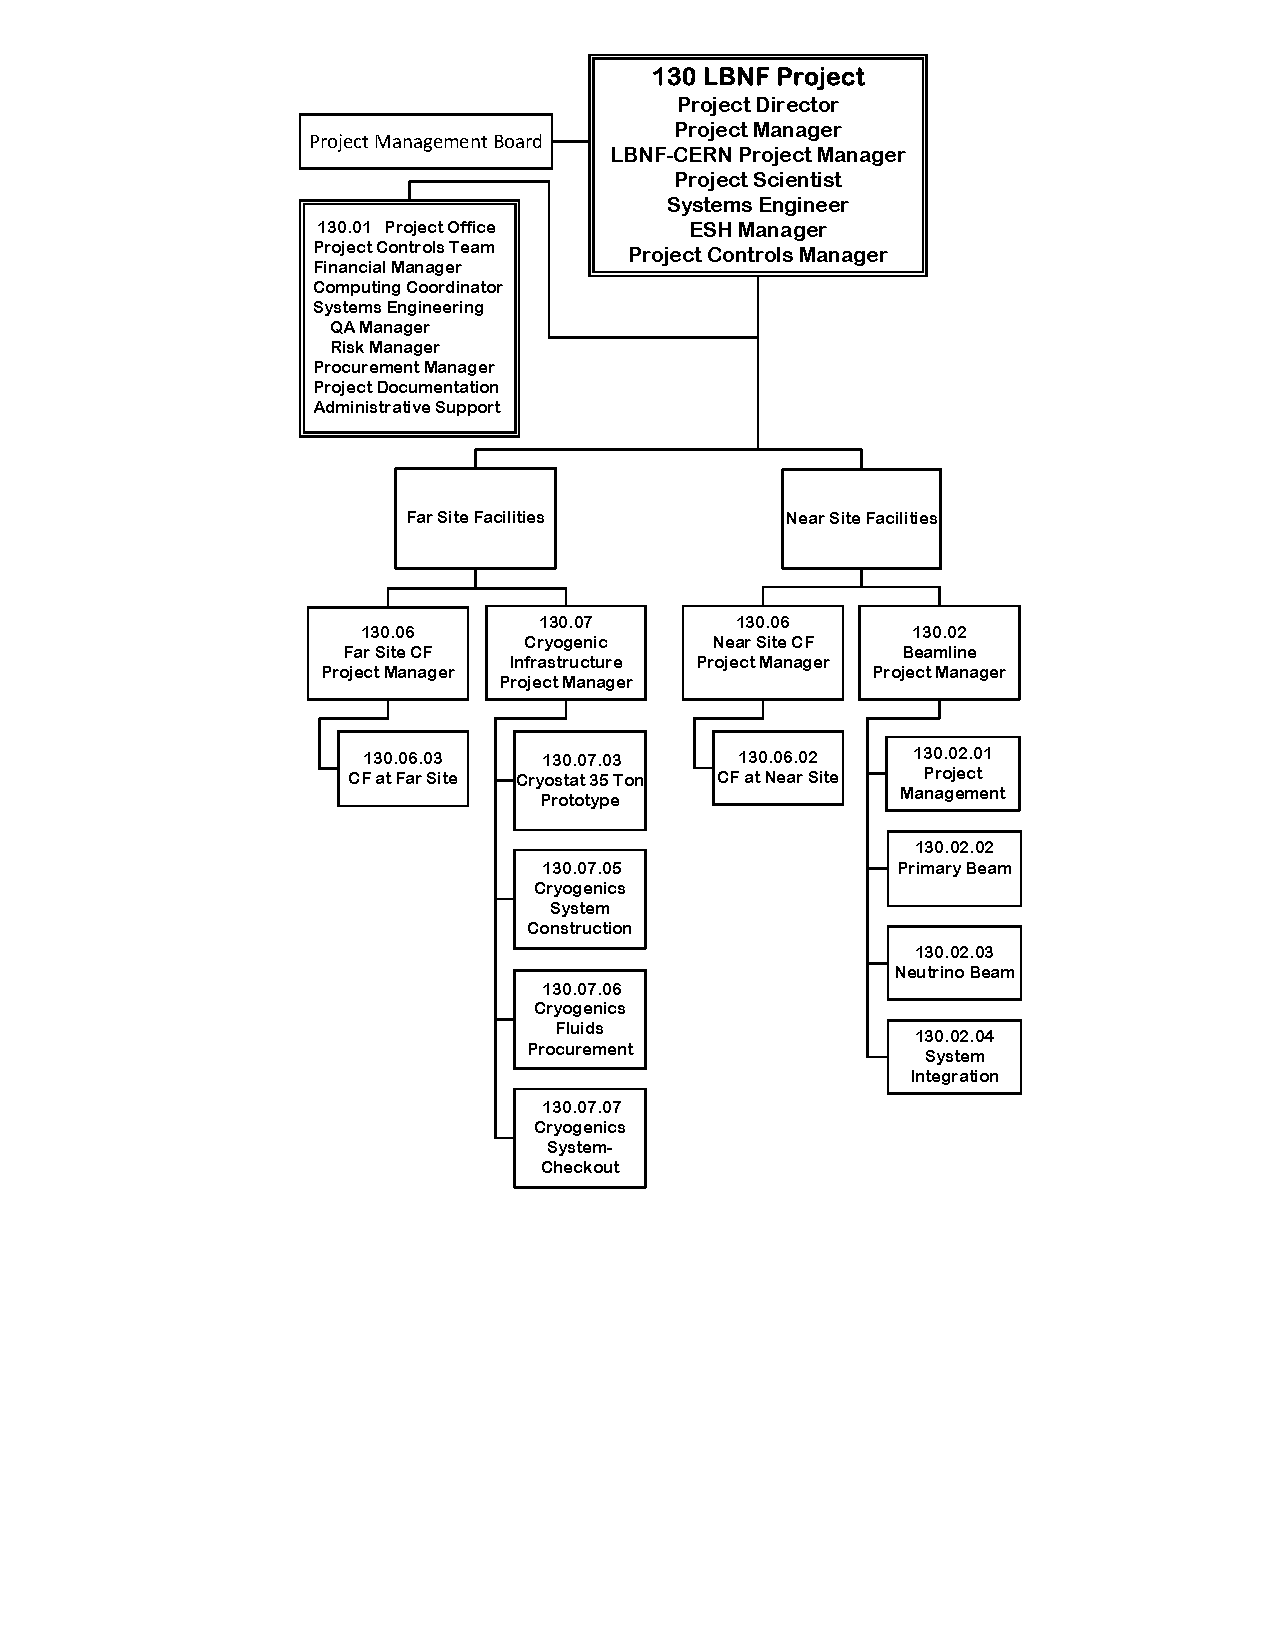
\includegraphics[width=0.8\textwidth]{lbnf-org-to-level3}
\end{cdrfigure}

Through their delegated authority and in consultation with major stakeholders, the L2 Project Managers appoint the WBS Level~3 Managers and also determine which of their lower-tier managers will be Control Account Managers (CAMs) for the Project WBS. L2 and L3 Project Managers are directly responsible for generating and maintaining the cost estimate, schedule, and resource requirements for their Projects and for meeting the goals of their Projects within the accepted baseline cost and schedule. 


\begin{cdrfigure}[LBNF Work Breakdown Structure to WBS Level 3]{lbnf-wbs}{LBNF Work Breakdown Structure to WBS Level 3}
  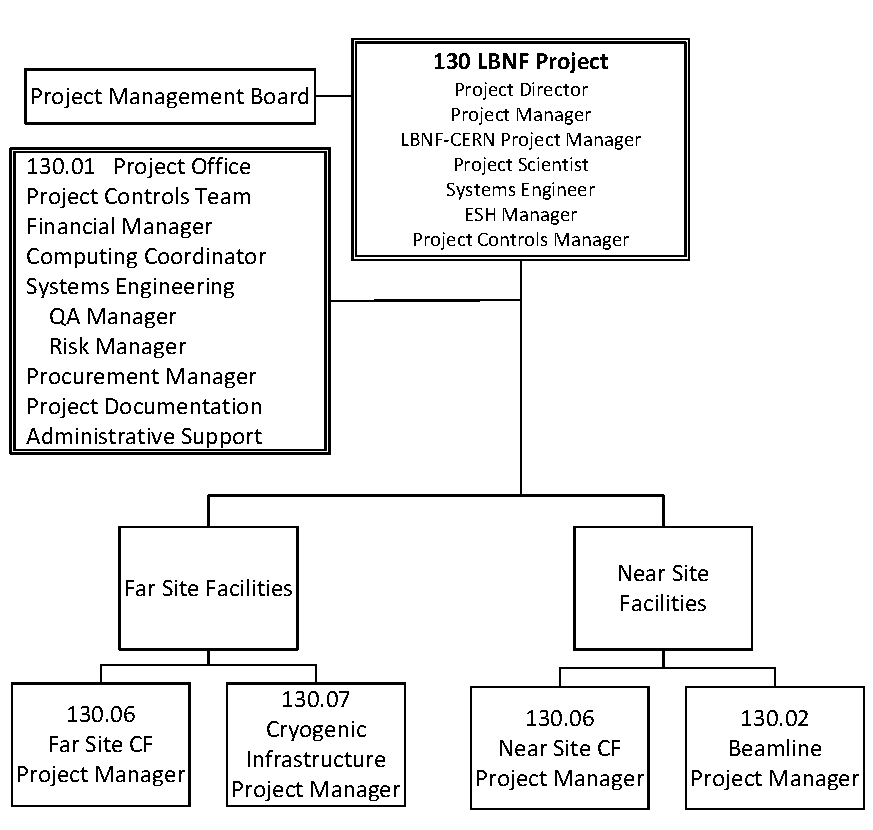
\includegraphics[width=0.8\textwidth]{lbnf-wbs-to-level3}
\end{cdrfigure}

The design and construction of LBNF is supported by other laboratories and consultants/contractors that provide scientific, engineering and technical expertise. A full description of LBNF Project Management is contained in the LBNF Project Management Plan \fixme{[ref]}.

%%%%%%%%%%%%%%%%%%%%%%%%%%%%%%%
\subsection{Fermilab}

\fixme{Some intro text about how Fermilab is the Near Site...}

%%%%%%%%%%%%%%%%%%%%%%%%%%%%%%%
%\subsection{South Dakota Science and Technology Authority and SURF}
\subsection{SDSTA and SURF}

LBNF plans to construct facilities at SURF to house the DUNE far detector. This facility is owned by the state of South Dakota and managed by the South Dakota Science and Technology Authority (SDSTA). \fixme{define SURF, SDSTA earlier}

Current SURF activities include operations necessary to to allow safe access to the 4850L for the existing and under-development science experiments. DOE is presently funding SDSTA ongoing operations through Lawrence Berkeley National Laboratory (LBNL) and its SURF Operations Office through FY16; this is expected to change to funding through Fermilab starting in FY17. 

The LBNF Far Site Facilities Manager is also an employee of SDSTA and is contracted to Fermilab to provide management and coordination of the Far Site Facilities CF and Cryo Infrastrastrucre. The LBNF Project also contracts directly with SDSTA to provide the management and design of LBNF Conventional Facilities at SURF; consruction for the CF will be directly contracted from Fermilab. Coordination with SDSTA and the LBNF Project is necessary to ensure efficient operations at SURF while meeting LBNF requirements. This will be facilitated via an agreement being developed between SDSTA and Fermilab regarding the LBNF Project \fixme{[new reference]} that defines responsibilities and methods of working together during the LBNF Project design and construction. A separate agreement will be written for LBNF Operations. 

%%%%%%%%%%%%%%%%%%%%%%%%%%%%%%%
\subsection{CERN}

The European Organization for Nuclear Research (CERN) will participate in the LBNF Project by providing cryogenic facilities and equipment to support the far detector and some technical components for the beamline. As a key CF %Facilities 
partner, CERN will provide the design and production, as well as coordinate with others in LBNF for the installation for identified deliverables. CERN engineers and scientists will participate in LBNF as assigned managers for specific scope as outlined %in the sections 
below. 

Details of the agreements with CERN will be contained in \fixme{[name the agreements here]}.  

%%%%%%%%%%%%%%%%%%%%%%%%%%%%%%%
\subsection{Coordination within LBNF}


The LBNF Project line organization is headed by the LBNF Project Director who is also the Fermilab Deputy Director for LBNF and reports to the Fermilab Director. The Project Director heads two divisions 
\fixme{are these `divisions' formal entities? If so, they need more of an introduction and should be Divisions. If not, I would just say: ``The Project Director heads both the Far Site Facilities and Near Site Facilities} 
that align with the LBNF L2 Projects: Far Site Facilities and Near Site Facilities. At the time of CD-1 Refresh Review, this organization is %transitioning (! )
%\fixme{you don't ``transition into existence;'' you could say ``personnel are transitioning into this organization''}
coming into existence and is expected to be in place in Fall 2015. Personnel who are working more than half time on the project are expected to be in these divisions while others may be matrixed part-time as required from other Fermilab Divisions/Sections/Centers or may work on LBNF as requested. Fermilab D/S/C Heads work with the L1 and L2 Project Managers to supply resources on an annual basis. 

The LBNF WBS defines the scope of the work. All changes to the WBS must be approved by the LBNF Project Manager prior to implementation. At the time of CD-1-Refresh, the LBNF WBS is in transition. Both the current and the post CD-1-R WBS is shown in Figure~\ref{fig:lbnf-wbs} to demonstrate how the scope will map from one WBS to the other. 

SDSTA assigns engineers and others as required to work on specific tasks required \fixme{add something about ``at the SURF site''} for LBNF. This is listed in the resource-loaded schedule as contracted work from Fermilab for Far Site CF activities. 

CERN and Fermilab are developing a common cryogenics team for LBNF as well as other liquid argon engineering activities. CERN assigns engineers and other staff as required to accomplish LBNF cryo infrastructure tasks. 



\fixme{Something about ``LBNF has formed several management groups with responsibilities as described below.''}

\textbf{Project Management Board:} LBNF uses a Project Management Board to provide formal advice to the Project Director on matters of importance for the LBNF Project as a whole. Such matters include (but are not limited to) those that:
\begin{itemize}
\item have significant technical, cost or schedule impact on the Project
\item have impacts on more than one L2 Project
\item affect the management systems for the Project
\item have impacts on or result from impact from other Projects on which the LBNF is dependent
\item result from external reviews or reviews called by the PD
\end{itemize}
The Management Board serves as the
\begin{itemize}
\item LBNF Change Control Board, as described in the Configuration Management Plan \fixme{[ref]}
\item Risk Management Board, as described in the Fermilab Risk Management Plan  \fixme{[ref]}
\end{itemize}

\textbf{Beamline Technical Board:} The role of the LBNF Beamline Technical Board is to provide recommendations and advice to the Beamline Project Manager on important technical decisions that affect the design and construction of the Beamline. The members of the Technical Board must have knowledge of the Project objectives and priorities in order to perform this function. The Beamline Project Manager chairs the Beam TB. The Beamline Project Engineer is the Scientific Secretary of the Board and co-chairs the Beam TB as needed. 

\textbf{FSCF Neutrino Cavity Advisory Board:} The FSCF Project has engaged three international experts in hard rock underground construction to advise it periodically through the design and construction process regarding excavation at SURF. The board meets at the request of the FSCF-PM, generally on site to discuss specific technical issues. The board produces a report with its findings and conclusions for project information and action. 



%%%%%%%%%%%%%%%%%%%%%%%%%%%%%%%%%%%%%%%%%%%%%%%%%%%%%
\section{DUNE}

%%%%%%%%%%%%%%%%%%%%%%%%%%%%%%
\subsection{DUNE Collaboration Structure}

The DUNE Collaboration brings together the members of the international science community 
interested in participating in the DUNE experiment.  The Collaboration defines the scientific goals of the experiment and subsequently 
the requirements on the experimental facilities needed to achieve these goals.  The Collaboration also provides the scientific and 
technical effort required for the design and construction of the DUNE detectors, operation of the experiment, and analysis of the 
collected data. There are four main elements in the DUNE organizational structure:  
\begin{itemize}
\item the DUNE Collaboration, composed of the General Assembly of the collaboration and the DUNE Institute Board     
\item DUNE Management, composed of the two co-spokespersons, the Technical Coordinator (TC), the Resource Coordinator (RC), who along
  with the IB chair and five other members of the collaboration form the DUNE Executive Committee (EC)
\item the DUNE Project Office (PO)
\item the DUNE Science Team, led by the Physics and Software/Computing coordinators. 
\end{itemize}
The relationships between these entities is illustrated in Figure~\ref{fig:dune-org}.

\begin{cdrfigure}[DUNE Project and Collaboration Organization]{dune-org}{DUNE Project and Collaboration Organization}
  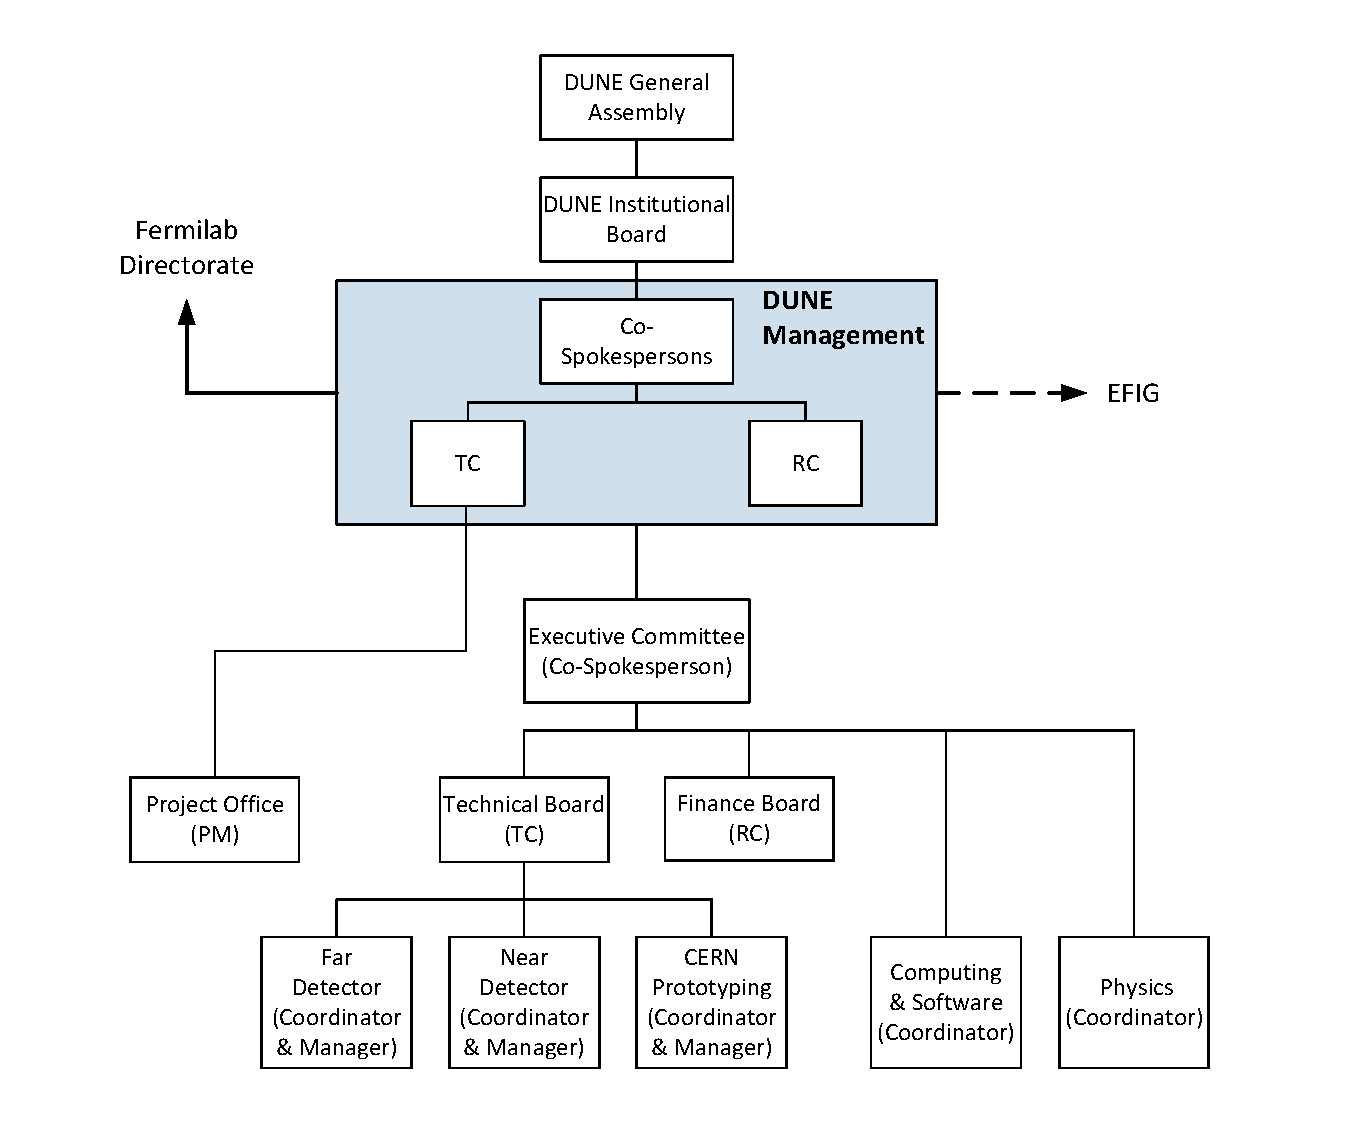
\includegraphics[width=0.95\textwidth]{dune-collaboration-org}
\end{cdrfigure}

\fixme{(for Anne) command to keep figure from floating ...}
\begin{cdrfigure}[DUNE Work Breakdown Structure]{dune-wbs}{DUNE Work Breakdown Structure}
  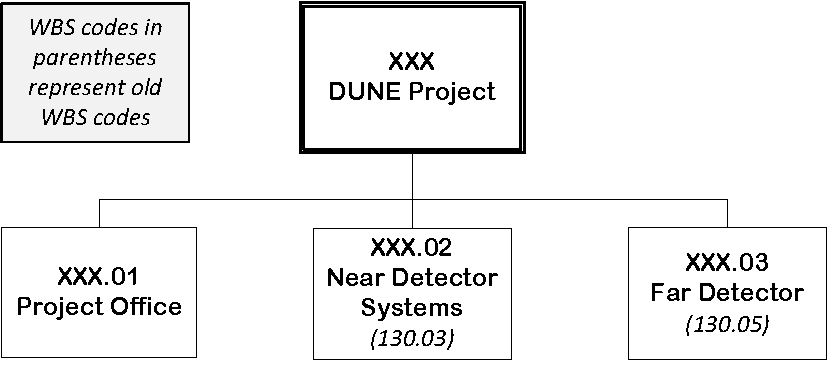
\includegraphics[width=0.8\textwidth]{dune-wbs-to-level3}
\end{cdrfigure}

%%%%%%%%%%%%%%%%%%%%%%%%%%%%%%
\subsection{Responsibilities of the DUNE Leadership}

The main responsibilities of the different roles are summarized below:
\begin{itemize}
  \item \textbf{The DUNE General Assembly} is composed of all members of the collaboration, it is consulted on major strategic decisions 
    through open plenary sessions at collaboration meetings and is informed through regular collaboration phone calls;
  \item \textbf{The DUNE Institutional Board} represents the institutes of the collaboration. It is composed of one representative from each 
    of the member institutions and has responsibility for Collaboration governance.  The IB has final authority over Collaboration 
    membership issues and defines requirements for inclusion of individuals within the DUNE authorship list. The IB is also responsible    
    for establishing and monitoring the process through which the co-spokespeople are selected to serve as leaders of the collaboration.   
  \item \textbf{The DUNE co-spokespersons} are accountable to the collaboration. They 
    are responsible for the day-to-day running of the collaboration and for representing the collaboration to Fermilab, funding 
    agencies and the broader scientific community.
  \item \textbf{The DUNE Executive Committee (EC)} is chaired by the longest serving co-spokesperson and is the primary 
    decision-making body of the collaboration. Membership of the EC includes the co-spokespeople, DUNE Project Office leaders, IB 
    chair, and five additional Collaboration members (three elected IB representatives and two additional members selected by the co-
    spokespeople). The EC will work by consensus. In the cases where consensus cannot be reached, 
    the authority lies with the spokespeople. If the co-spokespeople disagree, the TC will arbitrate.
  \item \textbf{The Technical Coordinator (TC)} reports to the spokespersons and the Fermilab director. 
     The TC acts as the project director 
    and is responsible for the implementation of the scientific and technical strategy of the collaboration through the DUNE project office.
    The TC is also responsible for the management of the DOE contributions to the DUNE project.  
     The Technical Coordinator prepares and chairs the meetings of the Technical Board of the experiment collaboration.
     \item \textbf{The Technical Board (TB)} discusses and approves the technical planning for all subsystems of the DUNE detector;
       \item \textbf{The Resource Coordinator (RC)} reports to the spokespersons and the Fermilab director. The RC
    The Resources Coordinator is responsible for coordinating the financial planning and other
resources issues of the collaboration. The Resource Coordinator is responsible in particular for
the management of the common resources of the Collaboration (common fund).
The Resources Coordinator prepares and chairs the meetings of the Finance Board (internal) of
the experiment collaboration. The Resources Coordinator is responsible for the
preparation of the Memoranda of Understanding of the Collaboration.
    \item \textbf{The Finance Board (FB)} is responsible for dealing with matters related to
the costs and resources of the Collaboration, evaluation of the contributions, relations with the
funding agencies and all administrative matters.  
    \item \textbf{The DUNE Science Team} is led by the physics coordinator and the software/computing coordinator and is responsible for the management of the DUNE scientific WGs;
    \item \textbf{The DUNE Project Office (PO)} provides the project management for the design, construction, installation, and commissioning of the DUNE near and far detectors. DUNE will be run as an international project matching DOE requirements. This will imply maintaining a full cost and schedule for the entire project, from which the DOE-funded portion can be extracted and monitored in a manner that satisfies DOE reporting requirements. The DUNE Project Office will have direct control over DOE project funds and any common fund collected from the U.S. and international stakeholders. International contributions to DUNE will be in the form of deliverables as defined in formal Memoranda of Understanding (MOU). These contributions will be tracked through detailed sub-project milestone. The entire Project (including international contributions) will be subject to the DOE critical decision process incorporating a CD-2 approval of its baseline cost and schedule and a CD-3 approval for moving forward with construction.  The high-level WBS structure of the Project is illustrated in Figure~\ref{fig:dune-wbs}.
    \item \textbf{The DUNE Technical WGs} The organization of the technical working groups of the DUNE collaboration is the responsibility of the L2 managers in the DUNE project.
\end{itemize}



%%%%%%%%%%%%%%%%%%%%%%%%%%%%%%%%%%%%%%%%%%%%%%%%%%%%%
\section{LBNF/DUNE Interfaces and Coordinating Bodies}
\label{sec:lbnf-dune-interface}

\fixme{Eric to add some text here} 
Figure~\ref{fig:lbnfdune-org} ... shows the upper level control and interfaces between the LBNF and DUNE Projects.  The role of each box...described here... 

\begin{cdrfigure}[LBNF/DUNE Project Structure]{lbnfdune-org}{LBNF/DUNE Project Structure}
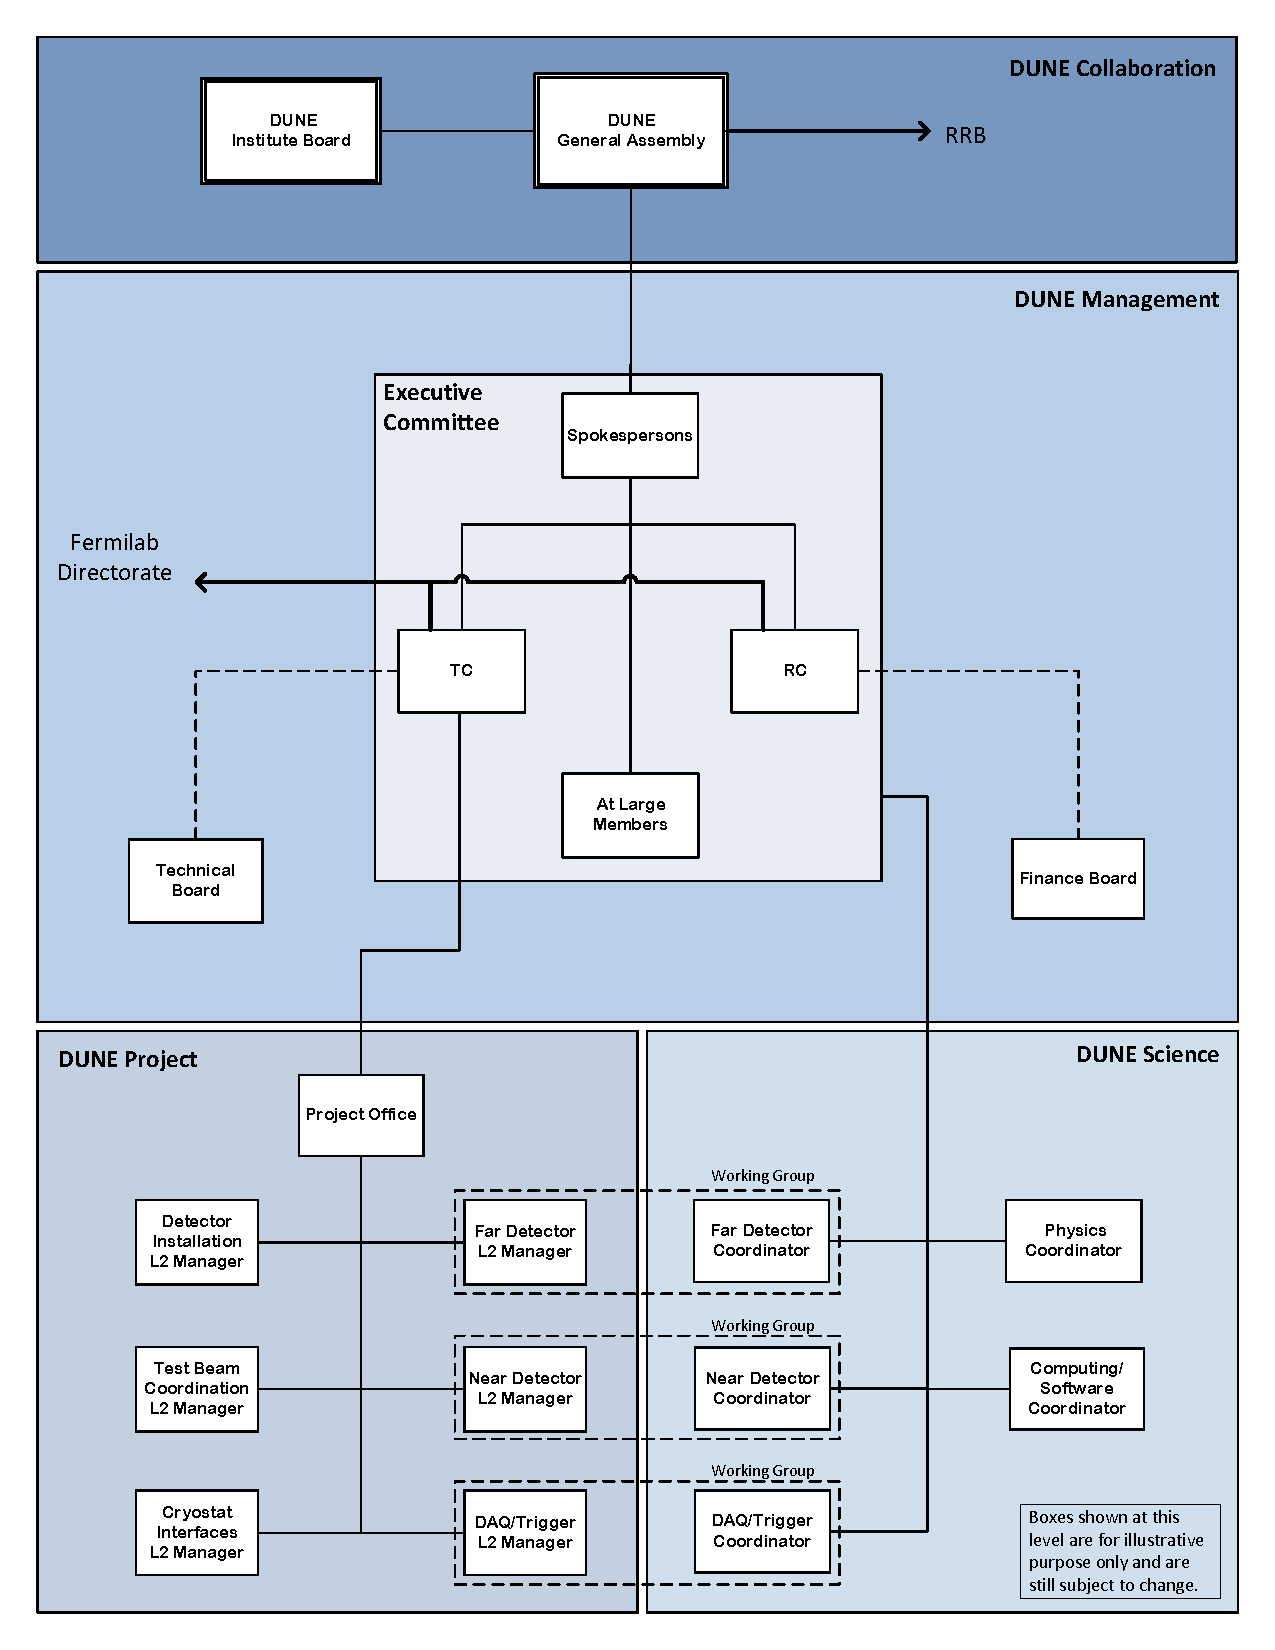
\includegraphics[width=0.8\textwidth]{lbnf-dune-structure}
\end{cdrfigure}

\subsection{International Advisory Committee (IAC) }

The International Advisory Committee (IAC) provides primary oversight and coordination of the two projects.  This group is made up representatives from each of the funding agencies involved in the program and provides global coordination across the entire enterprise.  In particular, this group is responsible for developing a plan that divides the financial responsibilities for constructing the facilities and detectors.   This group also has a leading role in developing the bi-lateral and subsidiary agreements between the DOE and other international stakeholders required to advance the program. 

\subsection{Fermilab, the Host Laboratory}

As the host laboratory, Fermilab has a direct responsibility for the design, construction, commissioning, and operation of the facilities and infrastructure that support the program.  In this capacity, Fermilab reports directly to the    DOE through the Fermilab Site Office (FSO).   Fermilab also has an important oversight role for the DUNE project itself as well as an important coordination role in ensuring that interface issues between the two projects are completely understood.  The following mechanisms will be used to ensure performance of Fermilab’s oversight and coordination roles. 

\subsection{LBNC Advisory Committee}

	The LBNC is an international, external advisory committee tasked with providing peer review for the two projects.  This group monitors the projects through regular meetings with the management teams and provides guidance   to the Fermilab director in his oversight role.  The Fermilab director appoints the head of this committee, who is then responsible for appointing additional committee members. \fixme{The LBNC Advisory Committee body needs to be distinguished better from the IAC; e.g., if the IAC is more about funding, is this more about science?}


\subsection{Resource Research Board (RRB)}

 	This body serves as the operational arm of the International Advisory Committee.  The Fermilab Director in coordination with the DUNE resource coordinator defines its membership, which includes representatives of the funding agencies contributing to the projects.  The deputy lab director is the chair of the board and organizes regular meetings to ensure that the needed  flow of funding to the projects is maintained.  The RRB is charged with defining different national contributions to the projects and their associated Memoranda of Understanding.   It is also responsible for understanding in-kind contributions to common projects. 

\subsection{Experiment-Facility Interface Group (EFIG)}

	The EFIG is the official body tasked with coordinating the LBNF and DUNE projects.  The Fermilab director controls the membership of this group, and his deputy serves as its head.  Group membership includes members of the Fermilab management such as the Chief Project Officer, members of the LBNF project management team, the DUNE co-spokespeople, as well as the DUNE Technical and Resource Coordinators.  The director at his discretion appoints additional members to ensure fulfillment of the group’s function, which is to oversee and ensure the required coordination of the LBNF and DUNE projects during the design, construction, and operational phases of the program.    
	
\subsection{DUNE Collaboration}	

	The collaboration, in consultation with the Fermilab Director, is responsible for forming the international project team responsible for designing and constructing the detectors.  The Technical Coordinator (TC) and Resource Coordinator (RC) serve as the lead managers of this international project team and are selected jointly by the spokespeople and the Fermilab director.  Because the international project incorporates contributions from a number of different funding agencies, the international DUNE project is responsible for satisfying individual tracking and reporting requirements associated with each of the different contributions.  Collaboration oversight of the international project is accomplished through the following internal structures.


